%%%%%%%%%%%%%%%%%%%%  IDENTITY THEFT %%%%%%%%%%%%%%%%%%%%%%%%
\newpage
\subsection{Identity Theft}
\subsubsection{Lower Bound Computation}
\[
\begin{bmatrix}
\mathbf{x}_{\text{American Samoa}}^{(\text{count})}\\
\mathbf{x}_{\text{American Samoa}}^{(\text{dollars})}
\end{bmatrix}
=
\begin{bmatrix}
0 & \cdots & 0 & \cdots & 2\\
\$0 & \cdots & \$0 & \cdots & \$600
\end{bmatrix}.
\]
% Columns represent years 2016, \cdots, 2017, \cdots, 2022 for American Samoa Identity Theft.
% Raw counts: 2016=0, 2017=0, 2022=2.  Raw dollars: 2016=$0, 2017=$0, 2022=$600.
\[
\begin{bmatrix}
\mathbf{x}_{\text{American Samoa}}^{(\text{count scaled to sample population})}\\
\mathbf{x}_{\text{American Samoa}}^{(\text{dollars scaled to sample population})}
\end{bmatrix}
=
\begin{bmatrix}
0 & \cdots & 0 & \cdots & 8\\
\$0 & \cdots & \$0 & \cdots & \$2{,}100
\end{bmatrix}.
\]
% Per-capita scaled to Chattanooga population: 2016=0, 2017=0, 2022=8 victims; dollars: 2016=$0, 2017=$0, 2022=$2,100.
  \[
\bar{X}_{\text{American Samoa}}^{(m)}
= \frac{1}{N}\sum_{i=1}^{N} X_{\text{American Samoa},i}^{(m)},
\]
\\
\[
\qquad
m \in \{\text{scaled count},\text{scaled dollars}\}
\]
\[
\begin{bmatrix}
\bar{X}_{\text{American Samoa}}^{(\text{scaled count})}\\
\bar{X}_{\text{American Samoa}}^{(\text{scaled dollars})}
\end{bmatrix}
=
\begin{bmatrix}
2\\
\$300
\end{bmatrix}.
\]
\subsubsection{Upper Bound Computation}
\[
\begin{bmatrix}
\mathbf{x}_{\text{California}}^{(\text{count})}\\
\mathbf{x}_{\text{California}}^{(\text{dollars})}
\end{bmatrix}
=
\begin{bmatrix}
2{,}368 & \cdots & 2{,}609 & \cdots & 2{,}854\\
\$17{,}862{,}807 & \cdots & \$10{,}216{,}795 & \cdots & \$27{,}903{,}539
\end{bmatrix}.
\]
% Columns represent years 2016, \cdots, 2017, \cdots, 2022 for California Identity Theft.
\[
\begin{bmatrix}
\mathbf{x}_{\text{California}}^{(\text{count scaled to sample population})}\\
\mathbf{x}_{\text{California}}^{(\text{dollars scaled to sample population})}
\end{bmatrix}
=
\begin{bmatrix}
10 & \cdots & 11 & \cdots & 13\\
\$75{,}434 & \cdots & \$43{,}076 & \cdots & \$127{,}101
\end{bmatrix}.
\]
\[
\bar{X}_{\text{California}}^{(m)}
= \frac{1}{N}\sum_{i=1}^{N} X_{\text{California},i}^{(m)},
\]
\\
\[
\qquad
m \in \{\text{scaled count},\text{scaled dollars}\}
\]
\[
\begin{bmatrix}
\bar{X}_{\text{California}}^{(\text{scaled count})}\\
\bar{X}_{\text{California}}^{(\text{scaled dollars})}
\end{bmatrix}
=
\begin{bmatrix}
12\\
\$118{,}823
\end{bmatrix}.
\]
\subsubsection{Monte Carlo Simulations for Likelihood and Impact}
\begin{figure}[H]
  \centering
  \rotatebox{0}{\scalebox{1}{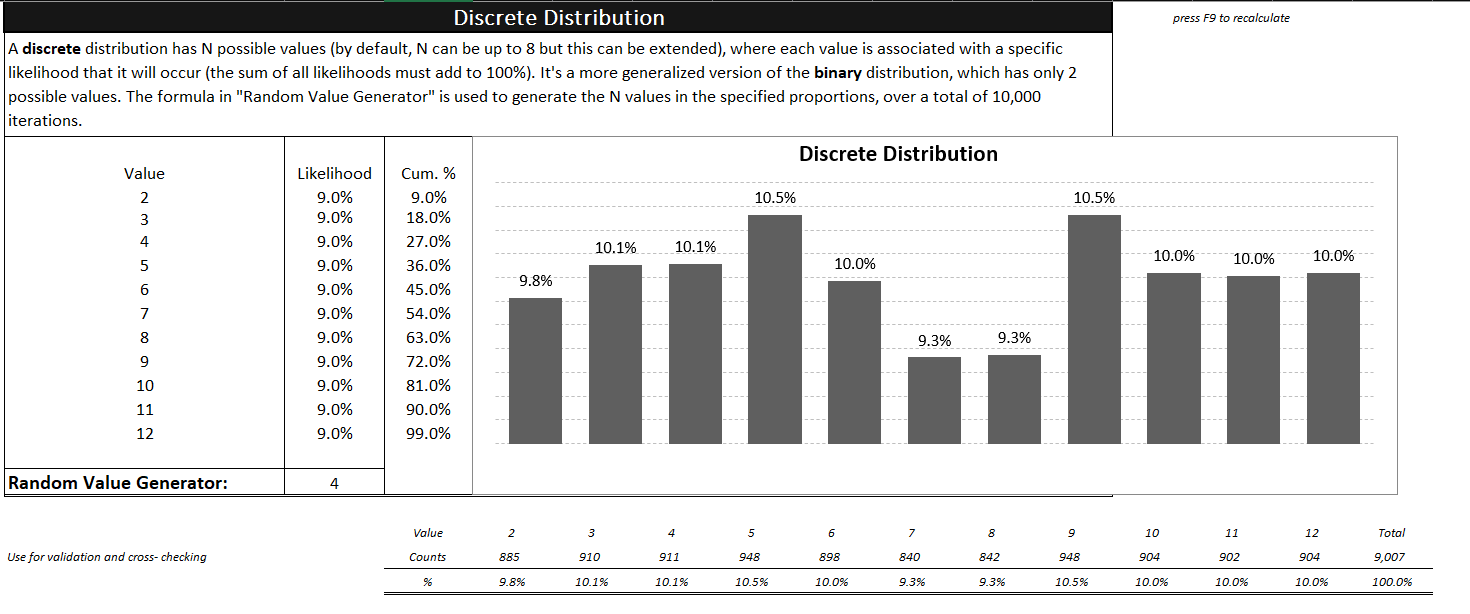
\includegraphics[scale=0.25]{figures/discrete_idtheft_count.png}}}
  \caption{We ran a\index{Monte Carlo simulation} Monte Carlo simulation of 10,000 iterations with a discrete distribution to spread random instances between confidence intervals taken from the means of seven year samples. We bounded between 2 and 12 possible \index{identity theft}identity theft events over a year.\protect\endnote{\index{sample} Sample size was set equivalent to the City of\index{Chattanooga} Chattanooga to determine the per capita rates for each year over data from \index{American Samoa} American Samoa and\index{California} California.  The means of those rates were used to set 10\% and 90\%\index{confidence interval} confidence intervals with \index{American Samoa} American Samoa and\index{California} California representing low and high \index{cybercrime} cybercrime counts respectively.}
  \protect\endnote{Monte Carlo Modeling Toolkit authored by Derek E. Brink, CISSP, \url{www.linkedin.com/in/derekbrink}. March 2023.}
  }
  \label{fig:screenshot-montecarlo-idtheft-count-discrete}
\end{figure}
When we computed the upper and lower bounds, we recognized that a normal distribution would not fit well for forecasting likelihood.  We took the mean of the sample from American Samoa for the lower bound (2); we took the mean from the sample from California for the upper bound (12); we had a separation of 10 units.  Therefore, we switched to a discrete model with all 11 options sharing an equal likelihood.
\begin{table}[H]
  \centering
  \caption{Monte Carlo Discrete Simulation Values for Identity Theft}
  \label{tab:discrete_idtheft_montecarlo}
  \begin{center}
  \begin{tabular}{@{}>{\centering\arraybackslash}
  p{0.20\linewidth} >{\centering\arraybackslash}
  p{0.10\linewidth} >{\centering\arraybackslash}
  p{0.10\linewidth} >{\centering\arraybackslash}
  p{0.10\linewidth} >{\centering\arraybackslash}
  p{0.10\linewidth} >{\centering\arraybackslash}
  p{0.10\linewidth} >{\centering\arraybackslash}
  p{0.10\linewidth}}
    \toprule
Events
&2
&3
&4
&5
&6
&7\\
    \midrule
Likelihood    
&8.9\%
&9.5\%
&9.1\%
&8.8\%
&9.4\%
&9.7\%\\
    \bottomrule \end{tabular}
\begin{tabular}{@{}>{\centering\arraybackslash}
  p{0.20\linewidth} >{\centering\arraybackslash}
  p{0.10\linewidth} >{\centering\arraybackslash}
  p{0.10\linewidth} >{\centering\arraybackslash}
  p{0.10\linewidth} >{\centering\arraybackslash}
  p{0.10\linewidth} >{\centering\arraybackslash}
  p{0.10\linewidth}}
    \toprule
Events    
    &8
    &9
    &10
    &11
    &12\\
    \midrule
Likelihood
&9.1\%
&9.4\%
&8.6\%
&8.3\%
&9.2\%\\
    \bottomrule \end{tabular}
    \end{center}
  \raggedright{A\index{Monte Carlo simulation} Monte Carlo simulation was run using a discrete distribution.  We bounded the simulation between 2 and 12 events.  We assigned a $\approx$9.1\% likelihood to each bin.  The resulting distribution showed the effect of randomness on each possible outcome.}
\end{table}

\begin{figure}[H]
  \centering
  \rotatebox{0}{\scalebox{1}{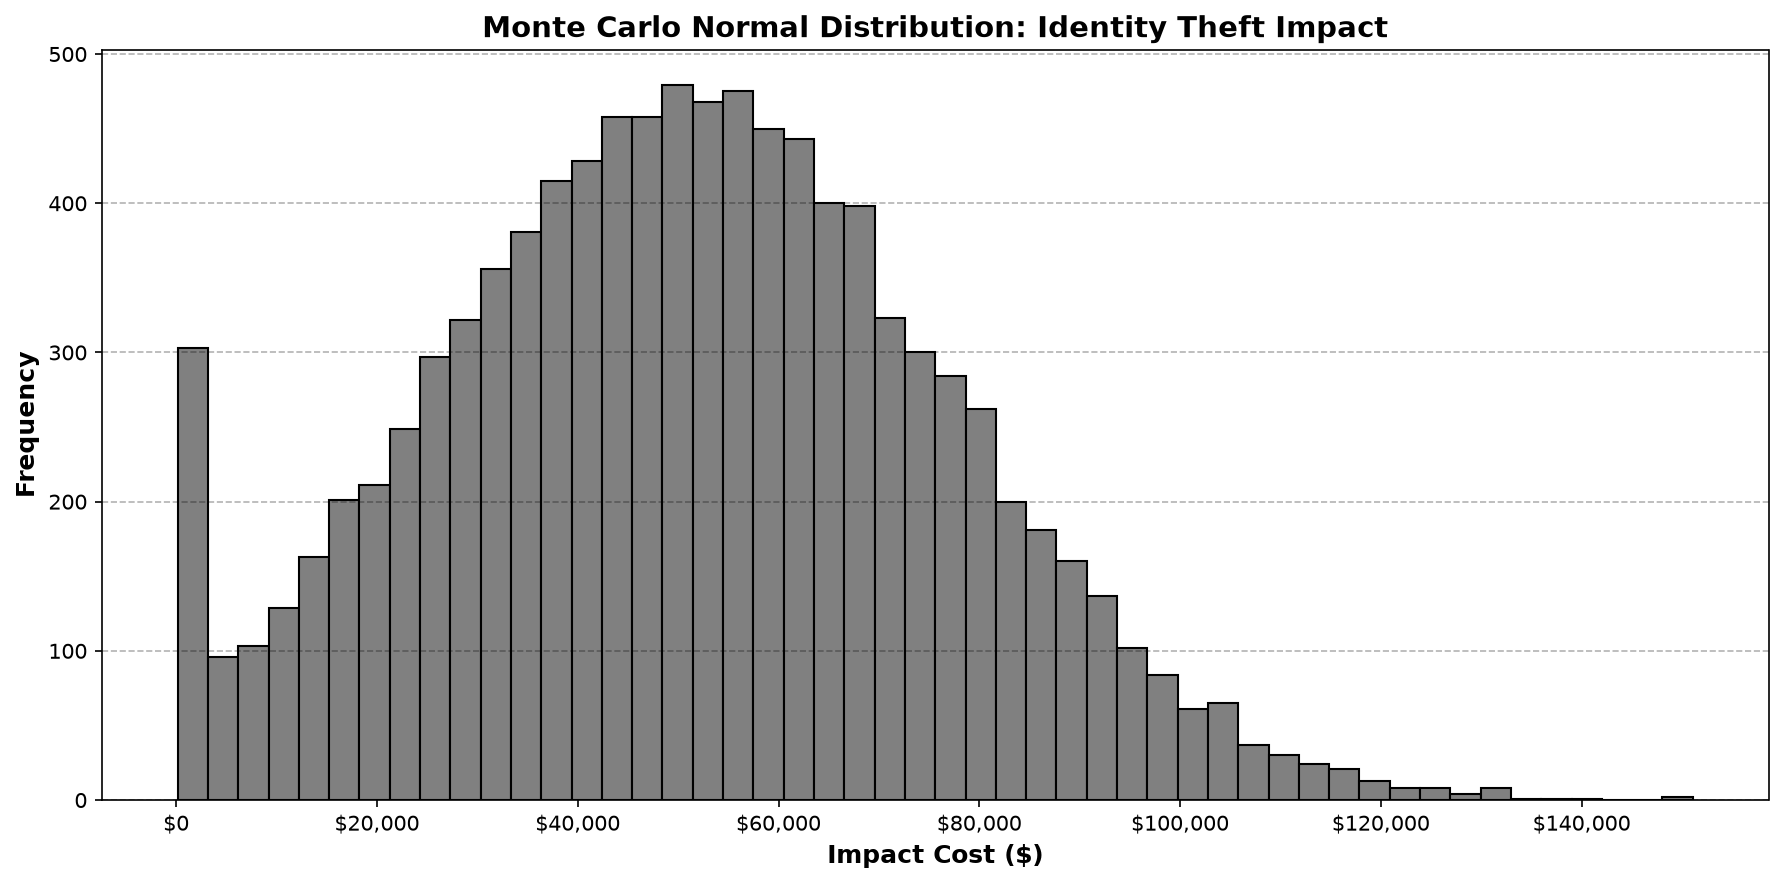
\includegraphics[width=\linewidth]{figures/histogram_idtheft_impact.png}}}
  \caption{We ran a\index{Monte Carlo simulation} Monte Carlo simulation of 10,000 iterations with a normal distribution to spread random instances between bounds taken from means of seven year samples. We set a lower bound that the events would cost at \$0.  We set an upper bound that the events would cost \$118{,}823.  \protect\endnote{\index{sample} Sample size was set equivalent to the City of\index{Chattanooga} Chattanooga to determine the per capita rates for each year over data from \index{American Samoa} American Samoa and\index{California} California.  The means of those rates were used to set upper and lower bounds with \index{American Samoa} American Samoa and\index{California} California representing low and high \index{cybercrime} cybercrime impact values respectively.}
  \protect\endnote{Monte Carlo Modeling Toolkit authored by Derek E. Brink, CISSP, \url{www.linkedin.com/in/derekbrink}. March 2023.}
  }
  \label{fig:screenshot-montecarlo-idtheft-impact-histo}
\end{figure}
\begin{figure}[H]
  \centering
  \rotatebox{0}{\scalebox{1}{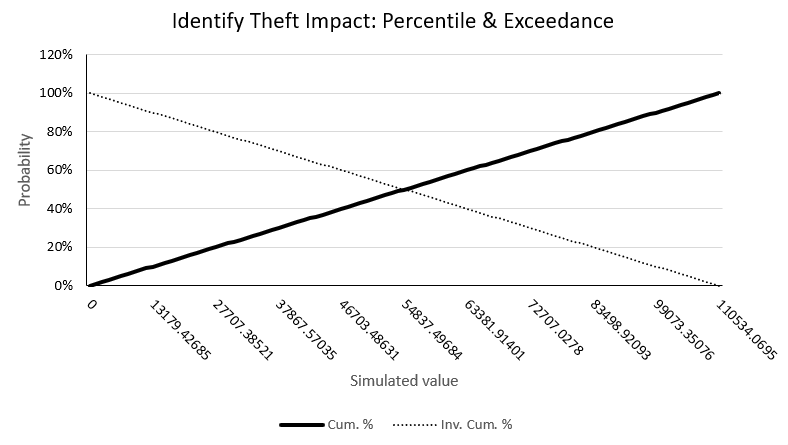
\includegraphics[width=\linewidth]{figures/percent_idtheft_impact.png}}}
  \[
\mathrm{CI}_{80\%}(\theta) = [\$12{,}668, \$98{,}880]
\]
  \caption{A\index{Monte Carlo simulation} Monte Carlo simulation with a normal distribution suggests that there is a 90\% probability that\index{identity theft} identity theft events will cost \$12{,}668 or more in a year.  There is a 50\% likelihood that they will cost \$56{,}158 or more in a year.  There is a 10\% chance that they will cost \$98{,}880 or more in a year. \protect\endnote{\index{sample} sample size was set equivalent to the City of\index{Chattanooga} Chattanooga to determine the per capita rates for each year over data from \index{American Samoa} American Samoa and\index{California} California.  The means of those rates were used to set 10\% and 90\%\index{confidence interval} confidence intervals with \index{American Samoa} American Samoa and\index{California} California representing low and high \index{cybercrime} cybercrime impact values respectively.}
  \protect\endnote{Monte Carlo Modeling Toolkit authored by Derek E. Brink, CISSP, \url{www.linkedin.com/in/derekbrink}. March 2023.}
  }
  \label{fig:screenshot-montecarlo-idtheft-impact-percent}
\end{figure}
